\documentclass{article}
\usepackage{amsmath,amsfonts,bm}
\usepackage{amsmath}
\usepackage[utf8]{inputenc}
\usepackage[T1]{fontenc}
\usepackage{xcolor}
\usepackage{tikz}
\usepackage{pgfplots}
\pgfplotsset{compat=1.17}
\usetikzlibrary{positioning}
\usetikzlibrary{calc}
\usetikzlibrary{pgfplots.groupplots}
\usetikzlibrary{external}

\begin{document}

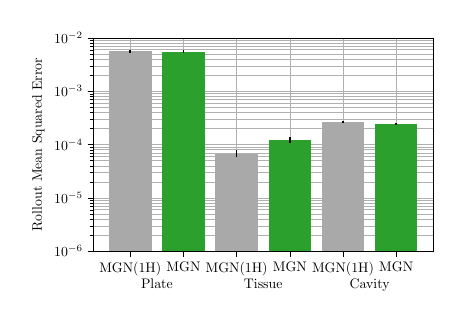
\begin{tikzpicture}[font=\normalsize, scale=0.5]

\definecolor{crimson2143940}{RGB}{214,39,40}
\definecolor{darkgray176}{RGB}{176,176,176}
\definecolor{darkorange25512714}{RGB}{255,127,14}
\definecolor{forestgreen4416044}{RGB}{44,160,44}
\definecolor{mediumpurple148103189}{RGB}{148,103,189}
\definecolor{sienna1408675}{RGB}{140,86,75}
\definecolor{steelblue31119180}{RGB}{31,119,180}
\definecolor{gray169}{RGB}{169,169,169}

\begin{axis}[
width=10.2cm,
height=7cm,
log basis y={10},
tick align=outside,
tick pos=left,
x grid style={darkgray176},
xmajorgrids,
xmin=-0.69, xmax=5.69,
xtick style={color=black},
xtick={0,1,2,3,4,5},
xticklabels={
MGN(1H),
MGN,
MGN(1H),
MGN,
MGN(1H),
MGN},
xticklabel style={align=center},
y grid style={darkgray176},
ylabel={Rollout Mean Squared Error},
ymajorgrids,
ymin=1e-06, ymax=0.01,
yminorgrids,
ymode=log,
extra x ticks ={0.5, 2.5, 4.5},
extra x tick labels={Plate, Tissue, Cavity},
extra x tick style={
    major tick length=1.4\baselineskip,
    major x tick style={draw=none},
    grid=none,
},
ytick style={color=black}
]
\draw[draw=none,fill=gray169] (axis cs:-0.4,1e-06) rectangle (axis cs:0.4,0.0055708650942202);

\draw[draw=none,fill=forestgreen4416044] (axis cs:0.6,1e-06) rectangle (axis cs:1.4,0.00550452694363064);

\draw[draw=none,fill=gray169] (axis cs:1.6,1e-06) rectangle (axis cs:2.4,6.7988724509875e-05);
\draw[draw=none,fill=forestgreen4416044] (axis cs:2.6,1e-06) rectangle (axis cs:3.4,0.000121950203180313);
\draw[draw=none,fill=gray169] (axis cs:3.6,1e-06) rectangle (axis cs:4.4,0.000264605454603831);
\draw[draw=none,fill=forestgreen4416044] (axis cs:4.6,1e-06) rectangle (axis cs:5.4,0.000246960852543513);
\path [draw=black, very thick]
(axis cs:0,0.00524432136464868)
--(axis cs:0,0.00589740882379171);

\path [draw=black, very thick]
(axis cs:1,0.00516381487138)
--(axis cs:1,0.00584523901588129);

\path [draw=black, very thick]
(axis cs:2,5.78538892222831e-05)
--(axis cs:2,7.81235597974668e-05);

\path [draw=black, very thick]
(axis cs:3,0.000106454943636323)
--(axis cs:3,0.000137445462724304);

\path [draw=black, very thick]
(axis cs:4,0.000252039437275171)
--(axis cs:4,0.000277171471932491);

\path [draw=black, very thick]
(axis cs:5,0.000236388867833816)
--(axis cs:5,0.000257532837253209);

\end{axis}

\end{tikzpicture}

\end{document}